\documentclass[11pt,a4paper]{article}
\usepackage[hyperref]{acl2020}
\usepackage{times}
\usepackage{latexsym}
\usepackage{graphicx}
\renewcommand{\UrlFont}{\ttfamily\small}

% This is not strictly necessary, and may be commented out,
% but it will improve the layout of the manuscript,
% and will typically save some space.
\usepackage{microtype}

\aclfinalcopy % Uncomment this line for the final submission
%\def\aclpaperid{***} %  Enter the acl Paper ID here

%\setlength\titlebox{5cm}
% You can expand the titlebox if you need extra space
% to show all the authors. Please do not make the titlebox
% smaller than 5cm (the original size); we will check this
% in the camera-ready version and ask you to change it back.

\newcommand\BibTeX{B\textsc{ib}\TeX}

\title{Instructions for ACL 2020 Proceedings}

\author{First Author \\
  Affiliation / Address line 1 \\
  Affiliation / Address line 2 \\
  Affiliation / Address line 3 \\
  \texttt{email@domain} \\\And
  Second Author \\
  Affiliation / Address line 1 \\
  Affiliation / Address line 2 \\
  Affiliation / Address line 3 \\
  \texttt{email@domain} \\}

\date{}

\begin{document}
\maketitle
\begin{abstract}
The most common way of working with existing transformers is to take a pre-trained model and add a ,,head'' on top of
that model for fine-tuning on various ML tasks, including semantical and syntactical tasks. In this paper we evaluate if the hidden states within a transformer are better for syntactical classification tasks (,,Part-of-Speech Tagging'') than the final layer.
\end{abstract}

\section{Introduction}

Increasing the amount of layers and thus total complexity of the model has shown great improvements across the entire range of machine learning tasks, including syntax tasks like POS-Tagging. But does a syntax task really require the same complexity as a semantic task? After all, understanding a sentence requires understanding the syntax as well.

\section{Methodology}

Using a pre-trained BERT model, we train a classifier by adding a linear classification head on top of the model.
In our experiment, we train multiple models with the classification head at different layers of BERT. This gives us 12 models to compare the performance of.

\section{Experiment}

Using the OntoNotesV4 dataset, for each layer, we fine-tune a pre-trained BERT model on a POS-Classification task with the classification head at that layer instead the final layer. We evaluate the F1 score of the models on 300 evaluation samples. Figure~\ref{fig:f1-full} shows Precision, Recall and F1 of every model trained on the full dataset. The models work fairly well ($F1 \approx 0.95$) at all layer counts. Models trained on 120 samples (Figure~\ref{fig:f1-120}) are less consistent but still fairly performant. Most importantly, even with only $\approx 4$ layers, a POS classifier has great performance.

\begin{figure}
\begin{center}
  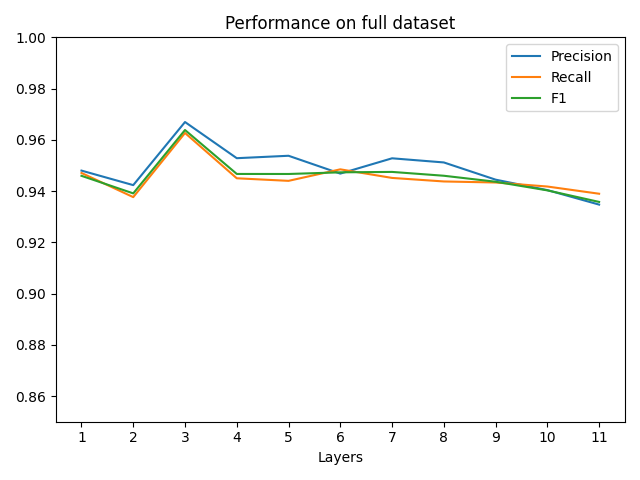
\includegraphics[width=\linewidth]{f1-full.png}
  % f1-full.png: 640x480 px, 72dpi, 22.58x16.93 cm, bb=0 0 640 480
  \caption{\label{fig:f1-full}F1 of whole dataset}
\end{center}
\end{figure}
\begin{figure}
\begin{center}
  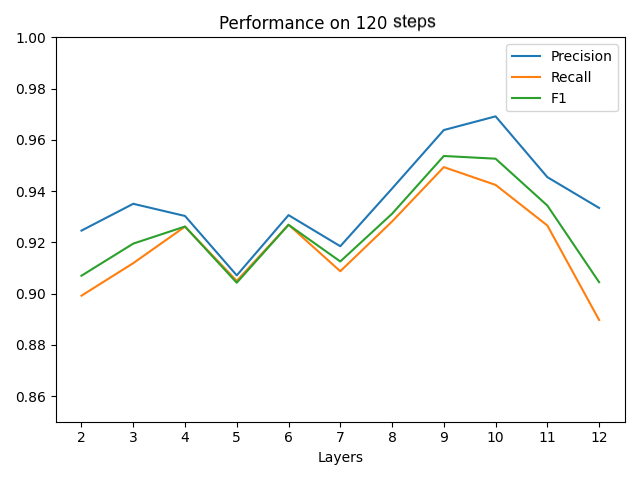
\includegraphics[width=\linewidth]{f1-120.png}
  % f1-full.png: 640x480 px, 72dpi, 22.58x16.93 cm, bb=0 0 640 480
  \caption{\label{fig:f1-120}F1 of 120 samples}
\end{center}
\end{figure}
\begin{figure}
\begin{center}
  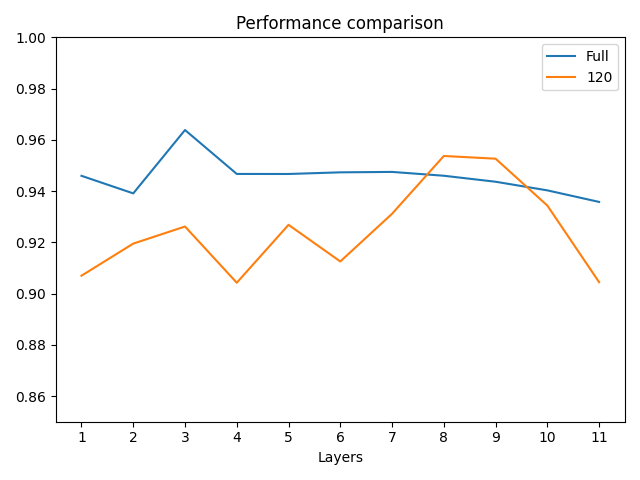
\includegraphics[width=\linewidth]{f1-comp.png}
  % f1-full.png: 640x480 px, 72dpi, 22.58x16.93 cm, bb=0 0 640 480
  \caption{\label{fig:f1-comp}F1 comparison}
\end{center}
\end{figure}

\end{document}
